\section{MÔ HÌNH CNN}
\subsection{Giới thiệu}
\subsubsection{Khái niệm cơ bản}
CNN (Convolutional Neural Network) là một kiến trúc mạng neural chuyên dụng cho xử lý dữ liệu có cấu trúc không gian như ảnh, video hoặc tín hiệu đa chiều. Khác với mạng neural truyền thống (DNN), CNN tập trung vào việc tự động trích xuất đặc trưng cục bộ thông qua các phép toán tích chập (convolution), giúp giảm đáng kể tham số mô hình mà vẫn đạt độ chính xác cao.
\subsubsection{Kiến trúc điển hình của CNN}

Một mô hình CNN cơ bản bao gồm các lớp chính sau:
\begin{figure}[H]
    \centering
    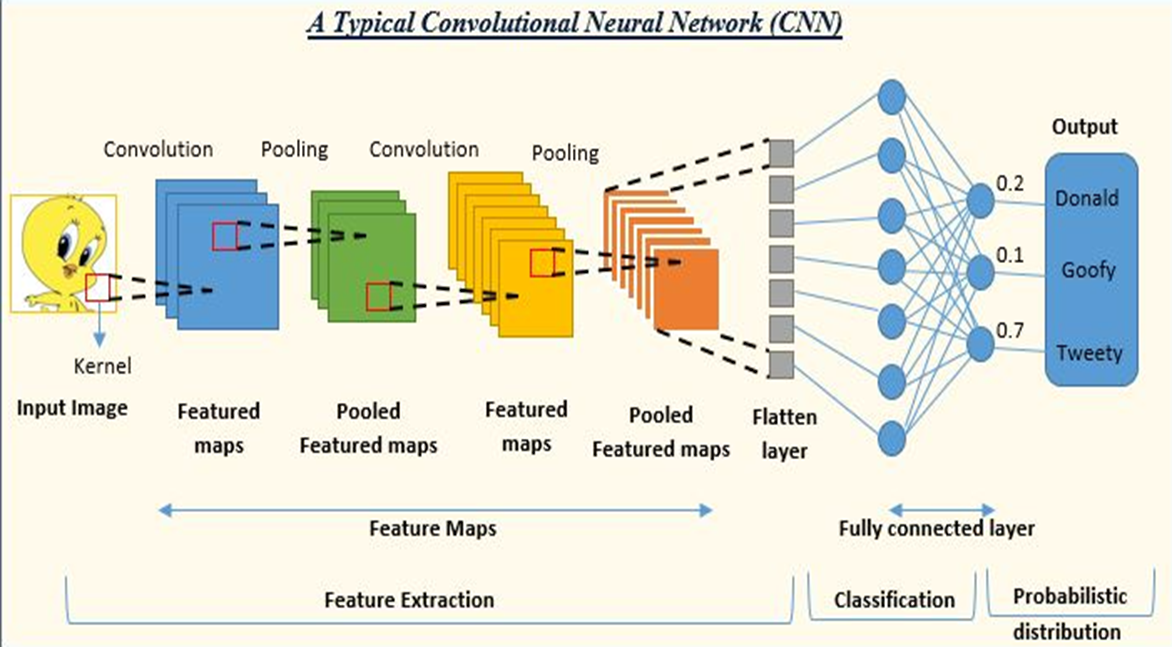
\includegraphics[width=0.9\linewidth]{Images/cnnarchi.png}
    \caption{Kiến trúc điển hình của CNN}
    \label{fig:enter-label}
\end{figure}

\begin{itemize}
    \item \textbf{Lớp Convolution (Conv):}
    \begin{itemize}
        \item Sử dụng bộ lọc (kernel) quét qua ảnh để phát hiện đặc trưng (ví dụ: cạnh, texture).
        \item Ví dụ: Kernel 3×3 với stride=1 và padding="same" giữ nguyên kích thước ảnh.
    \end{itemize}
    \item \textbf{Lớp Activation Function:} 
    \begin{itemize}
        \item ReLU (Rectified Linear Unit) là hàm kích hoạt phổ biến nhất, giúp mô hình hội tụ nhanh hơn.
        \item Sigmoid là một hàm kích hoạt phi tuyến có dạng chữ "S", biến đổi đầu vào thành khoảng giá trị từ 0 đến 1, thường được sử dụng trong các mô hình phân loại nhị phân để dự đoán xác suất.
    \end{itemize}
    \item \textbf{Lớp Pooling (Max/Average):}
    \begin{itemize}
        \item Giảm kích thước không gian (downsampling), tăng tính bất biến với nhiễu.
        \item Ví dụ: Max Pooling 2×2 giảm 50% kích thước ảnh.
    \end{itemize}
    \item \textbf{Lớp Fully Connected (FC):} Kết nối toàn bộ đặc trưng để phân loại (thường dùng ở cuối mô hình).
\end{itemize}
\subsubsection{Ưu điểm của CNN}
\begin{itemize}
    \item \textbf{Hiệu quả với dữ liệu ảnh:} Tận dụng tính chất cục bộ (local connectivity) và trọng số chia sẻ (shared weights), giảm overfitting.
    \item \textbf{Tiết kiệm tài nguyên:} Ít tham số hơn so với mạng DNN nhờ cơ chế convolution.
    \item \textbf{Khả năng mở rộng:} Dễ dàng kết hợp với các kiến trúc hiện đại (ResNet, Transformer).
\end{itemize}
\subsubsection{Ứng dụng điển hình}
\begin{itemize}
    \item \textbf{Nhận diện đối tượng:} Phát hiện khuôn mặt, chữ số viết tay (MNIST).
    \item \textbf{Phân đoạn ảnh y tế:} Xác định khối u trong ảnh MRI.
    \item \textbf{Xử lý video:} Theo dõi chuyển động trong camera an ninh.
\end{itemize}
\subsubsection{Biến thể nâng cao của CNN}
\begin{itemize}
    \item \textbf{ResNet:} Giải quyết vấn đề vanishing gradient bằng kết nối tắt (skip connection).
    \item \textbf{MobileNet:} Tối ưu cho thiết bị di động nhờ convolution tách rời (depthwise separable conv).
    \item \textbf{EfficientNet:} Cân bằng giữa độ chính xác và kích thước mô hình qua scaling coefficient.
\end{itemize}

\subsection{Xây dựng mô hình}
\textbf{Nền tảng thiết kế:} 
Mô hình CNN được đề xuất kế thừa các nguyên tắc cốt lõi từ AlexNet (khả năng trích xuất đặc trưng đa lớp với kernel lớn) và LeNet (kiến trúc đơn giản, phù hợp phần cứng), đồng thời để tối ưu hóa cho triển khai trên FPGA ta cần phải thay đổi mô hình theo các kỹ thuật sau.
\begin{figure}[H]
    \centering
    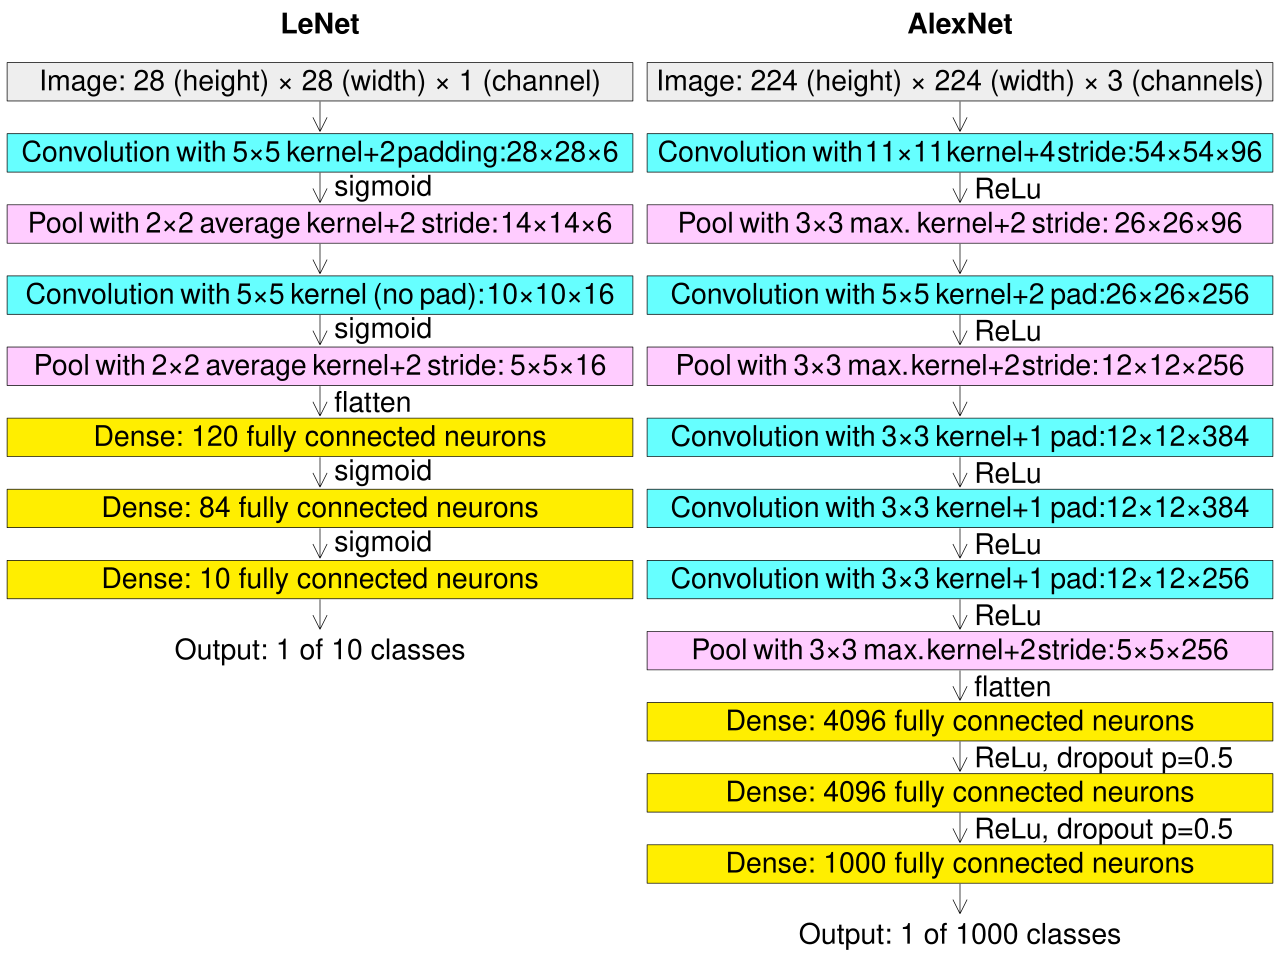
\includegraphics[width=0.75\linewidth]{Images/alexlenet.png}
    \caption{Cấu trúc mô hình LeNet và AlexNet}
    \label{fig:enter-label}
\end{figure}

\subsubsection{Xử lý đầu vào thực tế}
Tích hợp tiền xử lý ảnh trực tiếp trên FPGA (grayscale, resize về 28x28 như LeNet) để giảm latency. Và cũng phù hợp với Dataset MNIST đồ án này sử dụng để đào tạo mạng CNN.
\subsubsection{Thay thế và giảm bớt lớp fully connect}
Các mạng phổ biến cho nhận dạng chữ số viết tay bao gồm LeNet và AlexNet, những mạng này thường được sử dụng cho các tác vụ phân loại hình ảnh. Tuy nhiên, trong triển khai phần cứng, các mạng này có thể không phù hợp lắm do số lượng tham số lớn, vì vậy cần phải điều chỉnh các mạng này. Đặc biệt, các lớp fully connected yêu cầu rất nhiều trọng số (weight) và các bộ DSP. Ví dụ nếu số input fully connect là 100, output là 10 thì tổng số trọng số là 100x10 và 10 bias cho lớp fully connect này. 
\begin{figure}
    \centering
    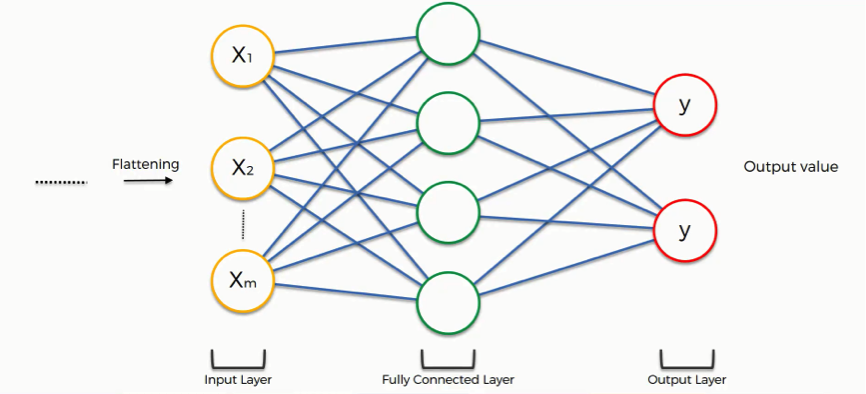
\includegraphics[width=0.75\linewidth]{Images/fullyconn.png}
    \caption{Fully connect}
    \label{fig:enter-label}
\end{figure}
Do đó để tiết kiệm tài nguyên triển khai, chúng ta cần giảm bớt trọng số của các lớp này. Một phương pháp phổ biến là sử dụng global max pooling để thay thế một phần trọng số của các lớp fully connected.
\begin{figure}[H]
    \centering
    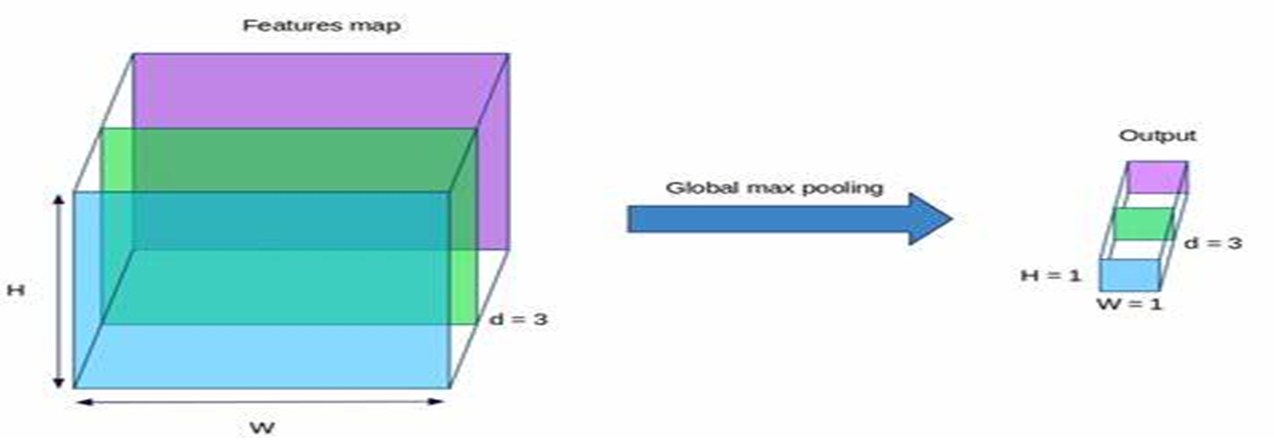
\includegraphics[width=0.75\linewidth]{Images/gmp.png}
    \caption{Global max pooling}
    \label{fig:enter-label}
\end{figure}
\subsubsection{Sử dùng hàm kích hoạt ReLU}
Hàm kích hoạt \textbf{ReLU} (Rectified Linear Unit) được định nghĩa:
\begin{equation}
    \text{ReLU}(x) = \max(0, x)
\end{equation}
\textbf{Lợi ích:}
\begin{itemize}
    \item \textbf{Tính toán hiệu quả}:
    \begin{equation}
        \text{Phép toán} \Rightarrow \begin{cases} 
        0 & \text{nếu } x < 0 \\
        x & \text{nếu } x \geq 0 
        \end{cases}
    \end{equation}
    Chỉ cần bộ so sánh (comparator) và multiplexer đơn giản
    
    \item \textbf{Tiết kiệm tài nguyên}:
    \begin{itemize}
        \item Không dùng phép nhân/phép chia phức tạp
        \item Chiếm ít LUTs (Look-Up Tables) trên FPGA
    \end{itemize}
    
    \item \textbf{Tận dụng pipeline}:
    $
        \text{Throughput} \uparrow \text{ nhờ latency thấp}
    $
    
    \item \textbf{Tương thích lượng tử hóa}:
    $
        \text{ReLU quan hệ tuyến tính} \Rightarrow \text{dễ dàng INT8/BNN hóa}
    $

\end{itemize}

\subsubsection{Binary Convolution (Tích chập nhị phân)}
Binary Weight Networks lượng tử hóa trọng số thành 2 giá trị $\{-1, +1\}$ nhưng giữ nguyên đầu vào full-precision. Công thức cơ bản:

\begin{equation}
    \mathbf{Y} = \mathbf{X} \ast \text{sign}(\mathbf{W})
\end{equation}

\noindent với:
\begin{itemize}
    \item $\mathbf{X}$: Đầu vào full-precision (float32)
    \item $\mathbf{W}$: Trọng số nhị phân hóa qua hàm $\text{sign}(\cdot)$
    \item $\ast$: Phép tích chập thông thường
\end{itemize}

\textbf{Quá trình nhị phân hóa}
\begin{equation}
    \text{sign}(W_{ij}) = \begin{cases} 
        +1 & \text{nếu } W_{ij} \geq 0 \\
        -1 & \text{nếu } W_{ij} < 0 
    \end{cases}
\end{equation}

\noindent Kèm theo scaling factor $\alpha$ để bù sai số:
\begin{equation}
    \alpha = \frac{1}{n} \|\mathbf{W}\|_1 = \frac{1}{n} \sum_{i,j} |W_{ij}|
\end{equation}

\textbf{Ưu điểm phần cứng}
\begin{itemize}
    \item \textbf{Tiết kiệm bộ nhớ}: Giảm 32x so với float32
    \item \textbf{Tối ưu phép nhân}: 
    \begin{equation}
        x \times \text{sign}(w) = \begin{cases} 
            +x & \text{nếu } w \geq 0 \\
            -x & \text{nếu } w < 0 
        \end{cases}
    \end{equation}
    \item Triển khai trên FPGA chỉ cần:
    \begin{itemize}
        \item Multiplexer chọn giữa $+x$ và $-x$
        \item Không cần DSP blocks cho phép nhân
    \end{itemize}
\end{itemize}

\textbf{Triển khai trên FPGA}
\begin{verbatim}
module binary_weight_layer (
    input [31:0] input_data,
    input binary_weight,
    output reg [31:0] result
);
    always @(*) begin
        result = (binary_weight == 1'b1) ? input_data : -input_data;
    end
endmodule
\end{verbatim}

\textbf{So sánh với Full-Precision và Xnor-net}
\begin{table}[h]
    \centering
    \begin{tabular}{|l|c|c|c|}
    \hline
    \textbf{Thông số} & \textbf{Full-Precision} & \textbf{Binary Weight} & \textbf{XNOR-Net} \\ \hline
    Bộ nhớ trọng số & 32 bit/parameter & 1 bit/parameter & 1 bit/parameter \\ \hline
    Bộ nhớ activations & 32 bit & 32 bit & 1 bit \\ \hline
    Phép toán nhân & Float multiplier & MUX + inverter & XNOR + popcount \\ \hline
    Tốc độ (FPGA) & 1x & 2.7x & 58x \\ \hline
    Độ chính xác & Baseline & Giảm 1-3\% & Giảm 8-12\% \\ \hline
    Năng lượng tiêu thụ & 100\% & 35\% & 12\% \\ \hline
    Scaling factor & Không cần & $\alpha$ cho weights & $\alpha$, $\beta$ cho activations \\ \hline
    Triển khai phần cứng & DSP blocks & LUTs + MUX & Pure LUTs \\ \hline
    \end{tabular}
\end{table}
\begin{figure}[H]
    \centering
    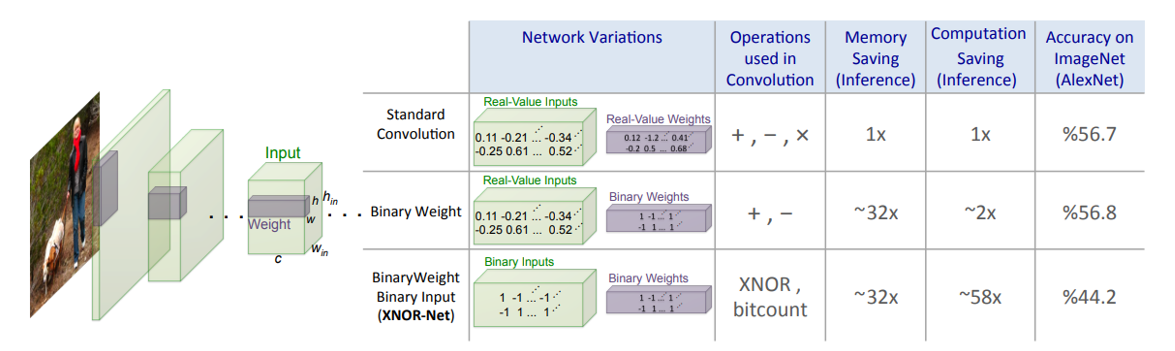
\includegraphics[width=0.9\linewidth]{Images/comparebinaryw.png}
    \caption{So sánh các phương pháp convolution}
    \label{fig:enter-label}
\end{figure}

\textbf{Xây dựng lớp Binary Convolution trên Tensorflow}
Vì Tensorflow không hỗ trợ sẵn nên ta cần phải dựa vào cấu trúc lớp Convolution mặc định để xây dựng lớp Binary Convolution. Với quá trình \textit{Forward} của lớp Convolution mặc định ta sẽ nhị phân hóa trọng số bằng cách sử dụng hàm \textit{tf.sign()}, giữ nguyên trọng số và \textit{Gradient} cho quá trình \textit{Backpropagation} để hội tụ nhanh hơn. 
\begin{lstlisting}[style=pythonstyle]
@tf.custom_gradient
def binarize(weights):
    """Function binarize weights with Straight-Through Estimator gradient"""
    def grad(dy, variables=None): 
        return dy  # Keep input gradient
    return tf.sign(weights), grad  # Binarize + custom gradient
\end{lstlisting}
\noindent\textbf{Giải thích:}
\begin{itemize}
    \item \texttt{@tf.custom\_gradient}: Decorator định nghĩa gradient tùy chỉnh
    \item \texttt{tf.sign(weights)}: Chuyển weights thành giá trị nhị phân $\{-1, 1\}$
    \item \texttt{grad(dy)}: Triển khai Straight-Through Estimator (STE) - truyền nguyên gradient đầu vào khi backpropagation
\end{itemize}

Với scaling-factor $\alpha$ để đơn giản phần lập trình ta đơn giản thay thế bằng cách thêm một lớp Batch Normalize sau lớp Binary Convolution. \\

Batch Normalization (BN) là kỹ thuật chuẩn hóa dữ liệu theo batch trong quá trình huấn luyện mạng neural, giúp ổn định và tăng tốc độ hội tụ.

\begin{equation}
    \hat{x}_i = \frac{x_i - \mu_B}{\sqrt{\sigma_B^2 + \epsilon}}
\end{equation}
\begin{equation}
    y_i = \gamma \hat{x}_i + \beta
\end{equation}


Trong đó:
\begin{itemize}
\item $\mu_B, \sigma_B^2$: Trung bình và phương sai của batch
\item $\gamma, \beta$: Tham số học được (scale và offset)
\item $\epsilon$: Hằng số tránh chia cho 0 (thường $10^{-5}$)
\end{itemize}
\textbf{Công dụng chính}
\begin{itemize}
    \item \textbf{Ổn định huấn luyện}: Giảm hiện tượng "internal covariate shift"
    \item \textbf{Hỗ trợ learning rate lớn}: Gradient ổn định hơn
    \item \textbf{Giảm phụ thuộc khởi tạo}: Ít nhạy cảm với giá trị ban đầu
    \item \textbf{Regularization ẩn}: Noise từ thống kê batch giảm overfitting
    \item \textbf{Tối ưu inference}: Sử dụng mean/variance cố định khi dự đoán
\end{itemize}

\subsection{Kết quả}
Từ cở sở trên ta xây dựng mô hình gồm 5 lớp Binary Convolution với sau mỗi lớp tích chập là khối Batch Normalize và Activation ReLU, 2 khối Max Pooling, 1 lớp Global Max Pooling và cuối cùng là 1 lớp Fully Connect.
\begin{figure}[H]
    \centering
    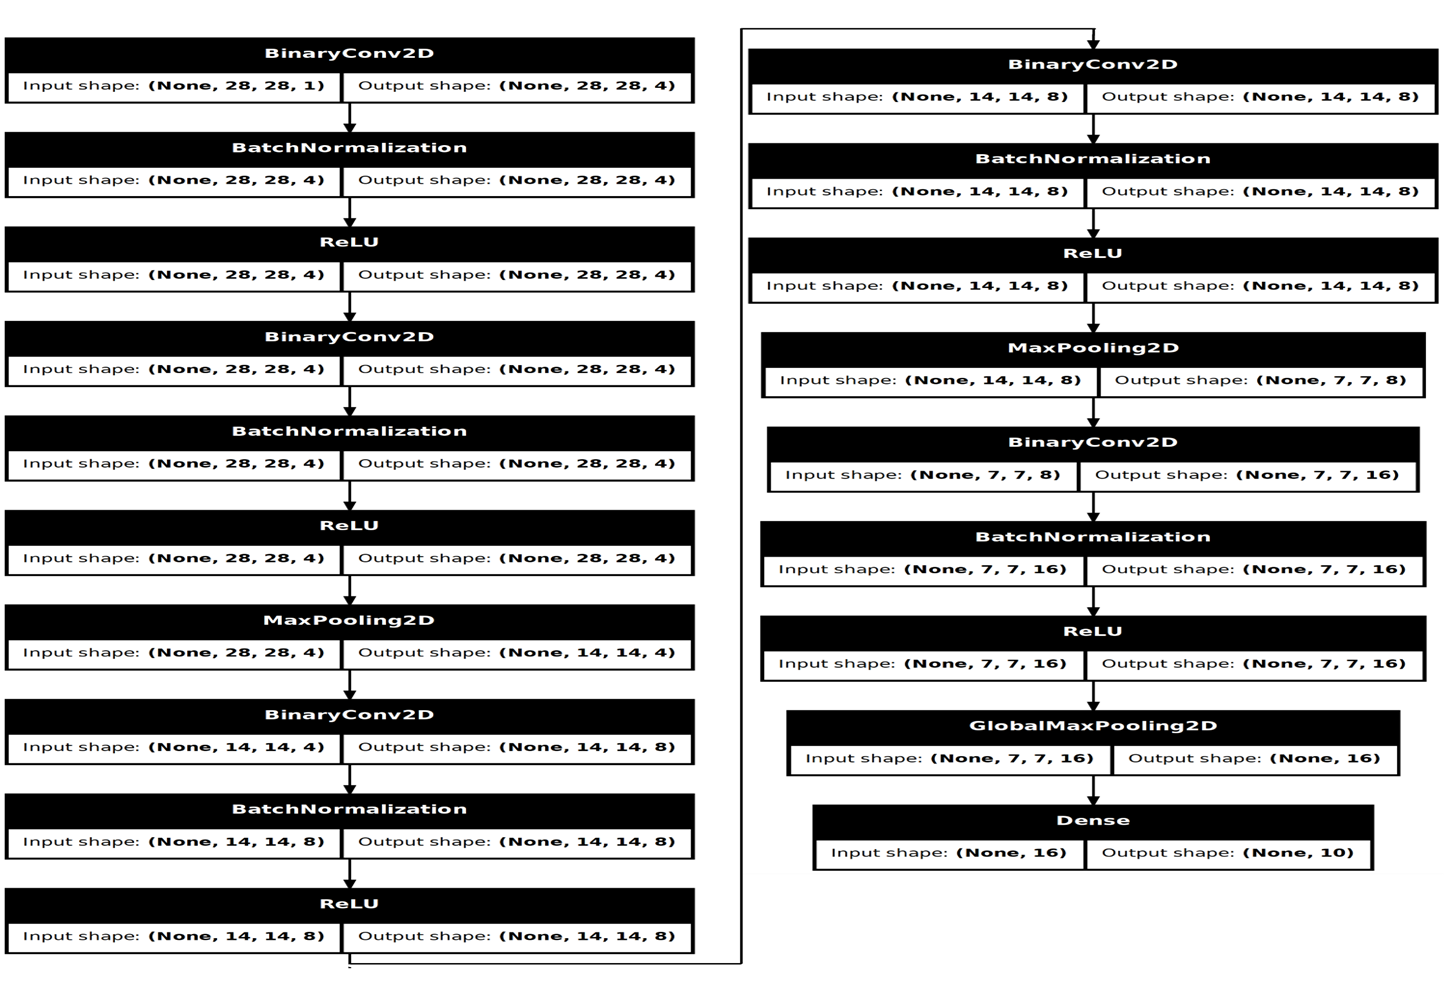
\includegraphics[width=1\linewidth]{Images/image.png}
    \caption{Model CNN}
    \label{fig:enter-label}
\end{figure}

\textbf{Kết quả training}
\begin{figure}[H]
    \centering
    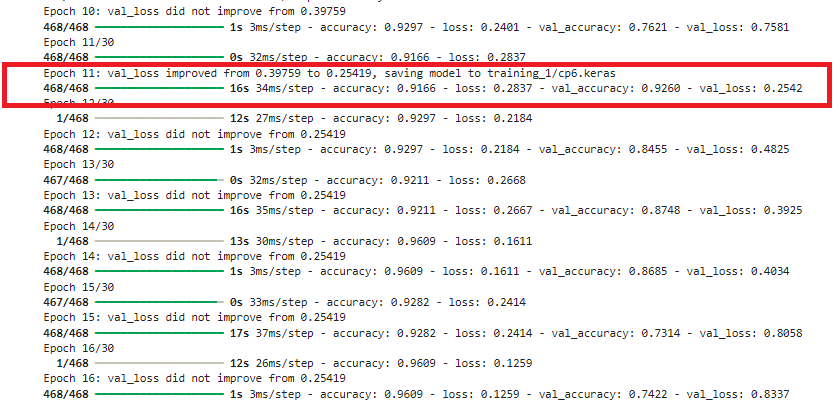
\includegraphics[width=0.9\linewidth]{Images/training.png}
    \caption{Kết quả training}
    \label{fig:enter-label}
\end{figure}
Quá trình training model sử dụng Adam optimizer với learning rate $10^{-4}$ có early stop ta có kết quả nhân diện đúng trên tập data \textit{Train} là $91.66\%$ loss $0.2873$ và kết quả trên tập data \textit{Evaluate} là $92.6\%$ loss $0.2542$
\begin{figure}[H]
    \centering
    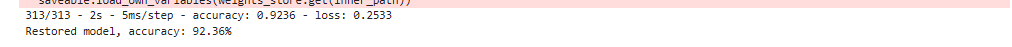
\includegraphics[width=0.9\linewidth]{Images/traintest.png}
    \caption{Kết quả test data MNIST}
    \label{fig:mnisttest}
\end{figure}
Kết quả test trên tập data \textit{Test} của MNIST có độ chính xác khoảng $92.36\%$.